\documentclass[conference]{IEEEtran}
\IEEEoverridecommandlockouts

\usepackage{cite}
\usepackage{amsmath,amssymb,amsfonts}
\usepackage{algorithmic}
\usepackage{algorithm}
\usepackage{graphicx}
\usepackage{tikz}
\usetikzlibrary{positioning,arrows.meta,fit,backgrounds,calc}
\usepackage{textcomp}
\usepackage{xcolor}
\usepackage{booktabs}
\usepackage{multirow}
% FIX 1: disable PDF bookmarks (EDAS rejects them) and keep coloured links
\usepackage[bookmarks=false,colorlinks=true,linkcolor=blue,citecolor=blue,urlcolor=blue]{hyperref}
% FIX 2: enforce margins that satisfy EDAS requirements
%   letter paper: right >= 0.57 in, top >= 0.70 in on all pages
\usepackage[letterpaper,
            left=0.68in, right=0.68in,
            top=0.75in,  bottom=1.00in,
            columnsep=0.21in,
            includeheadfoot=false]{geometry}

\def\BibTeX{{\rm B\kern-.05em{\sc i\kern-.025em b}\kern-.08em
    T\kern-.1667em\lower.7ex\hbox{E}\kern-.125emX}}

\begin{document}

\title{Sybil-Resistant Federated Learning via Blockchain-Based Economic Accountability}

\author{
    \IEEEauthorblockN{
        Ali Hamza\IEEEauthorrefmark{1}, 
        Xin-Jie Ye\IEEEauthorrefmark{2}, 
        Po-Kai Lu\IEEEauthorrefmark{2}, 
        Chih-Yi Chiu\IEEEauthorrefmark{2}, and 
        Chih-Hang Wang\IEEEauthorrefmark{2}
    }
    
    \IEEEauthorblockA{
        \IEEEauthorrefmark{1}\textit{National Research University Higher School of Economics}\\
        Moscow, Russian Federation\\
        \texttt{alihamza.369.2@gmail.com}
    }
    \vspace{0.2cm}
    
    \IEEEauthorblockA{
        \IEEEauthorrefmark{2}\textit{National Chung Cheng University}\\
        Chiayi County, Taiwan, R.O.C.\\
        \texttt{\{g13410124, g13410096, cychiu, chwang\}@ccu.edu.tw}
    }
}
\maketitle
\pagestyle{plain}
\begin{abstract}
Federated Learning (FL) in trustless, decentralized environments faces three critical vulnerabilities: susceptibility to Sybil attacks, model poisoning from adversarial participants. In addition, a widespread reliance on global validation sets that compromise data privacy. Likewise, the paper proposes a two-layer blockchain framework coupled with an EMH-DNN to address these challenges. Layer~1 implements Sybil-resistant identity governance through PoP registration and a decentralized median-voting PoC protocol. In addition, it eliminates the need for a shared global validation dataset. Similarly, Layer 2 monitoring relies solely on each committee member's private local test partition, with only aggregated metrics committed on-chain. Layer~2 introduces economic accountability via a staking mechanism and a blockchain-based state-rollback procedure that enables retroactive correction of poisoned model updates. The EMH-DNN architecture employs parallel feature-extraction branches with complementary dropout and client-specific output heads for shard-routing prediction under non-IID data distributions. Experimental evaluation on an approximate nearest neighbor routing task over the SIFT1B benchmark demonstrates that the framework maintains $\sim$93.8\% Recall@1000 under a 50\% Sybil attack across configurations of $N \in \{4, 8\}$ clients, while reducing the Attack Success Rate (ASR) from 100\% to 0.0\% through retroactive state correction.
\end{abstract}

\begin{IEEEkeywords}
Federated Learning, Blockchain, Sybil Attack, Model Poisoning Defense, Proof-of-Personhood, State Rollback
\end{IEEEkeywords}

%=====================================================
\section{Introduction}
%=====================================================

FL enables distributed clients to collaboratively train a shared model without exchanging raw data~\cite{li2020blockchain, kim2020ondevice}. However, the standard FL depends on a central server for aggregation -- a single point of failure, trust, and control. \emph{Blockchain-based FL} replaces this server with a decentralized ledger: clients train locally and submit model updates as blockchain transactions, where a consensus mechanism validates and aggregates contributions into a new global model. Similarly, it provides immutability (updates cannot be tampered with), auditability (every update is recorded), and decentralization (no single entity controls aggregation)~\cite{jiang2024bfl, li2022bflsurvey}--properties essential for privacy-sensitive applications where participants may not trust one another.

\textbf{Evolution and limitations of the field.} Early blockchain-FL systems such as BlockFL~\cite{kim2019blockfl} and FLChain~\cite{liu2020flchain} demonstrated feasibility but employed flat architectures with no economic accountability or Sybil resistance. Similarly, Committee-based designs followed: BFLC~\cite{li2020blockchain} introduced cross-validation committees, while Biscotti~\cite{shayan2021biscotti} combined Proof-of-Federation with Multi-Krum, tolerating up to 48\% adversaries. VeryFL~\cite{li2025veryfl} added verifiable smart contracts, and VFChain~\cite{peng2022vfchain} and VerifBFL~\cite{bellachia2025verifbfl} explored verifiable computation via authenticated data structures and zk-SNARKs. Reliance on shared global validation data to score contributions undermines the fundamental privacy FL aims to provide.

Decentralized consensus mechanisms are fundamentally threatened by the Sybil attack. Specifically, a vulnerability in which a lone adversary generates numerous fictitious identities. Douceur~\cite{douceur2002sybil} proved that Sybil resistance is impossible without some form of identity verification, motivating PoP protocols~\cite{borge2017pop, siddarth2020pop, adler2024phc}. Within FL, FoolsGold~\cite{fung2020foolsgold} and FedSybil~\cite{samy2023fedsybil} detect Sybils via gradient similarity, but all such defenses are \emph{reactive}---they attempt post-entry detection that sophisticated adversaries can evade~\cite{fang2020local}.

On the aggregation front, robust rules such as Krum~\cite{blanchard2017krum}, coordinate-wise Median~\cite{yin2018byzantine}, FLTrust~\cite{cao2021fltrust}, and FLAME~\cite{nguyen2022flame} offer statistical guarantees, but \emph{catastrophically fail under non-IID data}~\cite{huang2024federated, karimireddy2022bucketing}, and optimized attacks~\cite{fang2020local, baruch2019little} consistently circumvent them. Likewise, an inherent arms race that statistical defenses alone cannot resolve~\cite{karimireddy2021history}.

Economic mechanisms have been explored in blockchain consensus (Casper FFG's accountable safety~\cite{buterin2019casper}; Polkadot's slashing~\cite{wood2014polkadot}) and FL incentives (DeepChain~\cite{weng2021deepchain}; Kang et al.'s contract theory~\cite{kang2019incentive}; BlockFLA~\cite{desai2021blockfla}), but none include \emph{model rollback}. Specifically, they penalize financially without correcting the poisoned model. Conversely, model recovery methods (FedRecover~\cite{cao2023fedrecover}, Crab~\cite{jiang2024crab}) restore clean states but operate centrally without financial deterrence. Game-theoretic defenses (FedGame~\cite{wu2023fedgame}) model adversarial dynamics but carry no real economic consequences.

\textbf{Three open problems.} Across this landscape, three critical gaps persist: \textbf{(P1)} contribution evaluation requires global validation sets, violating privacy; \textbf{(P2)} committed poisoned updates are irreversible on blockchain; \textbf{(P3)} validators face no economic consequence for approving malicious updates.

\textbf{Our approach.} This paper addresses all three problems through a two-layer architecture (Fig.~\ref{fig:system}). \textbf{Layer~1} solves \textbf{P1} by replacing global validation sets with a PoP identity gate and peer-to-peer median-voting consensus, where committee members evaluate updates using only their \emph{private local data}. \textbf{Layer~2} solves \textbf{P2} and \textbf{P3} by introducing economic staking---validators must lock collateral---and a blockchain-based rollback mechanism that reverts the ledger state upon detecting poisoning, making attacks both \emph{economically irrational} (stake is slashed) and \emph{technically reversible} (model state is restored). To handle non-IID data heterogeneity, the study proposes the EMH-DNN, a parallel-branch architecture with client-specific output heads that mitigates catastrophic forgetting at the routing layer during aggregation.

\begin{figure}[t]
\centering
\resizebox{\columnwidth}{!}{%
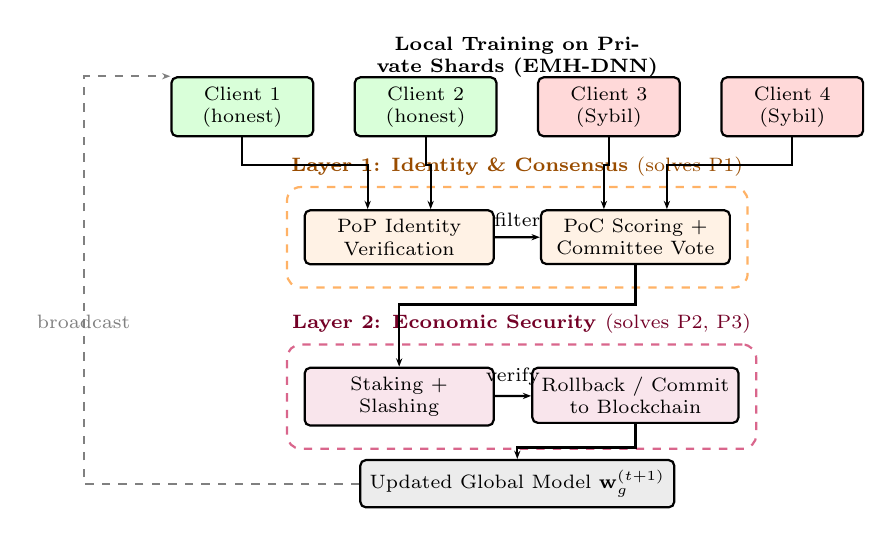
\begin{tikzpicture}[
    node distance=0.6cm and 0.4cm,
    clientbox/.style={rectangle, draw, thick, minimum width=1.8cm, minimum height=0.6cm, align=center, font=\scriptsize, rounded corners=2pt},
    sysblock/.style={rectangle, draw, thick, fill=blue!6, minimum width=2.4cm, minimum height=0.6cm, align=center, font=\scriptsize, rounded corners=2pt},
    layerbox/.style={rectangle, draw, dashed, thick, rounded corners=5pt, inner sep=6pt},
    arr/.style={-{Stealth[length=3pt]}, thick},
    lbl/.style={font=\scriptsize, text=black!70}
]

% === Row 1: Clients (evenly spaced) ===
\node[clientbox, fill=green!15] (c1) {Client 1\\(honest)};
\node[clientbox, fill=green!15, right=0.5cm of c1] (c2) {Client 2\\(honest)};
\node[clientbox, fill=red!15, right=0.5cm of c2] (c3) {Client 3\\(Sybil)};
\node[clientbox, fill=red!15, right=0.5cm of c3] (c4) {Client 4\\(Sybil)};

% Title above clients — FIX 7: constrain text width to prevent bounding-box overflow
\node[font=\scriptsize\bfseries, above=0.25cm of $(c2)!0.5!(c3)$,
      text width=5.5cm, align=center] (title)
      {Local Training on Private Shards (EMH-DNN)};

% === Row 2: Layer 1 — centered under clients ===
\coordinate (L1center) at ($(c2)!0.5!(c3)$);
\node[sysblock, fill=orange!10, below=1.3cm of L1center, xshift=-1.5cm] (pop) {PoP Identity\\Verification};
\node[sysblock, fill=orange!10, below=1.3cm of L1center, xshift=1.5cm] (poc) {PoC Scoring +\\Committee Vote};

% Layer 1 box
\node[layerbox, draw=orange!60, fit=(pop)(poc), inner ysep=8pt,
      label={[font=\scriptsize\bfseries, text=orange!60!black]above:Layer 1: Identity \& Consensus \textnormal{(solves P1)}}] (L1) {};

% === Row 3: Layer 2 — centered under Layer 1 ===
\node[sysblock, fill=purple!10, below=1.3cm of L1center, yshift=-2.0cm, xshift=-1.5cm] (stake) {Staking +\\Slashing};
\node[sysblock, fill=purple!10, below=1.3cm of L1center, yshift=-2.0cm, xshift=1.5cm] (roll) {Rollback / Commit\\to Blockchain};

% Layer 2 box
\node[layerbox, draw=purple!60, fit=(stake)(roll), inner ysep=8pt,
      label={[font=\scriptsize\bfseries, text=purple!60!black]above:Layer 2: Economic Security \textnormal{(solves P2, P3)}}] (L2) {};

% === Row 4: Global model — centered ===
\node[sysblock, fill=gray!15, below=0.8cm of $(stake)!0.5!(roll)$] (global) {Updated Global Model $\mathbf{w}_g^{(t+1)}$};

% === Arrows: Clients → Layer 1 (spread across PoP top) ===
\draw[arr] (c1.south) -- ++(0,-0.35) -| ([xshift=-0.4cm]pop.north);
\draw[arr] (c2.south) -- ++(0,-0.35) -| ([xshift=0.4cm]pop.north);
\draw[arr] (c3.south) -- ++(0,-0.35) -| ([xshift=-0.4cm]poc.north);
\draw[arr] (c4.south) -- ++(0,-0.35) -| ([xshift=0.4cm]poc.north);

% Layer 1 internal
\draw[arr] (pop) -- (poc) node[midway, above, font=\scriptsize] {filter};

% Layer 1 → Layer 2
\draw[arr] ($(poc.south)+(0,0)$) -- ++(0,-0.5) -| (stake.north);

% Layer 2 internal
\draw[arr] (stake) -- (roll) node[midway, above, font=\scriptsize] {verify};

% Layer 2 → Global
\draw[arr] (roll.south) -- ++(0,-0.3) -| (global.north);

% Feedback loop: Global → Clients (far-left vertical channel)
\draw[arr, dashed, black!50] (global.west) -- ++(-3.5,0) |- (c1.north west)
    node[pos=0.22, below, font=\scriptsize, text=black!50] {broadcast};

\end{tikzpicture}%
}
\caption{System workflow. Clients train locally using EMH-DNN and submit updates. Layer~1 filters Sybil identities via PoP and evaluates quality through committee-based PoC voting on private data (P1). Layer~2 enforces staking and triggers rollback upon detecting poisoning (P2, P3). The verified global model is broadcast for the next round.}
\label{fig:system}
\end{figure}

The principal contributions are: (1)~a \emph{two-layer trust architecture} integrating Sybil-resistant identity governance (Layer~1, addressing P1) with economic rollback security (Layer~2, addressing P2--P3); (2)~a \emph{privacy-preserving validation protocol} where committee members use only private local data, eliminating global validation sets; and (3)~a \emph{slashing-based accountability mechanism} with state rollback enabling retroactive correction of poisoned updates---a capability absent from all prior blockchain-FL frameworks~\cite{jebreel2023fl, alashhab2024enhancing, asiri2023understanding, jayagopal2023intrusion}.

%=====================================================
\section{Methodology}
%=====================================================

The research considers a decentralized network of $N$ clients that jointly minimize a global loss function $F(\mathbf{w})$ over their respective private datasets $\mathcal{D}_k$, $k = 1, \ldots, N$. The framework operates across two complementary security layers---Layer~1 for identity and consensus, Layer~2 for economic accountability---supported by the EMH-DNN architecture designed for non-IID robustness (Table~\ref{tab:symbols}).

% FIX 3: Table 1 used {ll|ll} which can overflow a single column.
%         Switch to tabularx or use fixed-width p{} columns.
\begin{table}[t]
\centering
\caption{Key Symbols and Parameters}
\label{tab:symbols}
\scriptsize
\setlength{\tabcolsep}{2pt}
\begin{tabular}{p{0.9cm}p{2.0cm}|p{0.9cm}p{2.0cm}}
\toprule
\textbf{Symbol} & \textbf{Definition} & \textbf{Symbol} & \textbf{Definition} \\
\midrule
$N$ & Total clients & $S_{PoC}$ & PoC score \\
$\tau_k^{(t)}$ & Trust score of $k$ at $t$ & $S_{min}$ & Min.\ stake \\
$\mathcal{C}^{(t)}$ & Committee at round $t$ & $P_{penalty}$ & Slashing penalty \\
$\mathbf{w}_k$ & Local weights of $k$ & $\delta_{drop}$ & Acc.\ drop threshold \\
$\mathbf{w}_g^{(t)}$ & Global model at $t$ & $\delta_{th}$ & PoC acceptance thr. \\
$Stake_k$ & Locked stake of $k$ & $\mathbf{z}$ & Fused feature repr. \\
$r_{reward}$ & Trust reward incr. & $r_{penalty}$ & Trust penalty decr. \\
$\tau_{min}$ & Full participation thr. & $H_k$ & Client-specific head \\
$\mathbf{W}_1,\mathbf{W}_2$ & Branch weight matrices & $B_1,B_2$ & Parallel branches \\
\bottomrule
\end{tabular}
\end{table}

\subsection{Layer 1: Identity Governance and Decentralized Consensus}

Layer~1 provides Sybil resistance and quality-aware model validation without requiring a global validation dataset.

\subsubsection{Trust Dynamics and Probation}

To prevent Sybil clients from immediately gaining full influence, every client $k$ maintains a dynamic trust score $\tau_k^{(t)} \in [0, 1]$, initialized at a low value $\tau_k^{(0)}$ through a Proof-of-Personhood (PoP) registration challenge. New clients enter a \emph{probationary state} below the full participation threshold $\tau_{min}$, ensuring they must demonstrate honest behavior before their updates carry significant weight. Trust evolves asymmetrically after each round:
% FIX 5: cases text was too wide for one IEEEtran column (~3.5 in).
%         Shortened right-side conditions; meaning is preserved in surrounding text.
\begin{equation}
\tau_k^{(t+1)} = 
\begin{cases} 
\min(1,\; \tau_k^{(t)} + r_{reward}) & \text{accepted \& honest} \\
\max(0,\; \tau_k^{(t)} - r_{penalty}) & \text{accepted \& malicious} \\
\tau_k^{(t)} & \text{rejected}
\end{cases}
\label{eq:trust}
\end{equation}

The asymmetry is deliberate: the reward increment $r_{reward}$ is small, so that reputation is earned gradually over many rounds, while the penalty $r_{penalty}$ is an order of magnitude larger, so that a single detected malicious act causes severe trust loss. This design follows the principle from PoS blockchain economics~\cite{buterin2019casper} that the cost of misbehavior must far exceed the cost of honest participation. Probationary clients receive a slightly higher reward rate to enable bootstrapping without granting premature influence. Clients below the minimum trust floor are excluded entirely, while those in probation ($\tau_k < \tau_{min}$) receive reduced aggregation weight (see Eq.~\ref{eq:agg}). Concrete parameter values are reported in Section~\ref{sec:config}.

\subsubsection{Committee Election and Peer Validation}

A validation committee $\mathcal{C}^{(t)}$ is elected each round via score-based selection, prioritizing clients with strong historical validation performance. Committee members must be PoP-registered and, when staking is enabled, hold sufficient stake. Members rotate each round to prevent concentration of validation power.

Because no global validation set exists, the committee evaluates each candidate update $\mathbf{w}_k$ using members' \emph{private local datasets}---the key mechanism that solves problem P1. To quantify update quality without shared data. The study introduces the PoC score. Likewise, which captures three complementary aspects of update utility:
\begin{equation}
S_{PoC}(k) = \gamma_1 \cdot u_{acc} + \gamma_2 \cdot u_{loss} + \gamma_3 \cdot u_{rob}
\label{eq:poc}
\end{equation}
where $u_{acc}$ measures the improvement in accuracy (how much the local update improves on the current global model), $u_{loss}$ captures the reduction in normalized losses (ensuring a scale-invariant comparison between clients), and $u_{rob} = (1 + \|\Delta\mathbf{w}\| / 100)^{-1}$ penalizes gradient explosions -- a known signature of poison attacks~\cite{fang2020local}. The coefficients $\gamma_1, \gamma_2, \gamma_3$ control the relative importance of accuracy, loss, and robustness.

An update must exceed a minimum PoC threshold $\delta_{th}$ and receive $\geq 2/3$ committee approval. The final contribution weight combines individual quality with the committee's aggregate median assessment:
\begin{equation}
S_{combined} = 0.6 \cdot S_{PoC} + 0.4 \cdot S_{median}
\label{eq:combined}
\end{equation}
Using the median (rather than the mean) ensures robustness to outlier evaluations from any compromised committee members, following the statistical guarantees of coordinate-wise median aggregation~\cite{yin2018byzantine}.

\subsection{Layer 2: Economic Security and Rollback}

Critically, no global dataset is introduced: each committee member independently evaluates the updated model on its own private local test partition, and the median Recall@1000 is computed on-chain — no raw data leaves any client. Layer~1's peer validation filters overtly malicious updates, but sophisticated poisoning attacks may pass initial quality checks yet degrade model performance over subsequent rounds. Layer~2 addresses this by making such attacks \emph{economically irrational} (solving P3) and \emph{technically reversible} (solving P2).

\subsubsection{Staking and Slashing}

The key insight, borrowed from PoS blockchain consensus~\cite{buterin2019casper}, is that validators who have financial skin-in-the-game are incentivized to verify honestly. Committee eligibility therefore requires locking a minimum stake $Stake_k \geq S_{min}$. When committee $\mathcal{C}^{(t)}$ approves a block $B_t$, members' stakes remain locked until the block's impact is verified. If global model quality $\text{Acc}_t$ drops below a safety margin $\delta_{drop}$ relative to the previous round, a \emph{slashing event} penalizes the responsible validators:
\begin{equation}
Stake_j \leftarrow \max(0,\; Stake_j - P_{penalty}), \quad \forall j \in \mathcal{C}^{(t)}
\label{eq:slash}
\end{equation}
Simultaneously, trust scores are reset to $\tau_j \leftarrow 0$, permanently banning the validators. The penalty $P_{penalty}$ is calibrated relative to $S_{min}$ so that a single slashing event eliminates a substantial fraction of stake, making the expected cost of approving a poisoned update exceed any potential gain from collusion.

\subsubsection{Blockchain Rollback}

Upon detecting poisoning, the rollback mechanism executes a three-step state reversion: (1)~invalidate block $B_t$, (2)~revert the global model to the last verified checkpoint $\mathbf{w}_g^{(t-1)}$, and (3)~resume training with a freshly elected committee. This capability directly addresses P2: unlike standard blockchain-FL where immutability makes corruption permanent, our ``time machine'' mechanism ensures that no single poisoned round can permanently compromise the global model.

\subsection{Model Architecture: Enhanced Multi-Head DNN}

To mitigate catastrophic forgetting under non-IID data distributions. The research introduces the EMH-DNN, which decouples shared feature extraction from client-specific routing prediction, isolating shard-level routing knowledge in dedicated output heads while relying on trust-weighted aggregation (Eq.~\ref{eq:agg}) to stabilize the shared representation. Figure~\ref{fig:arch} illustrates the complete architecture.

\begin{figure}[t]
\centering
\resizebox{\columnwidth}{!}{%
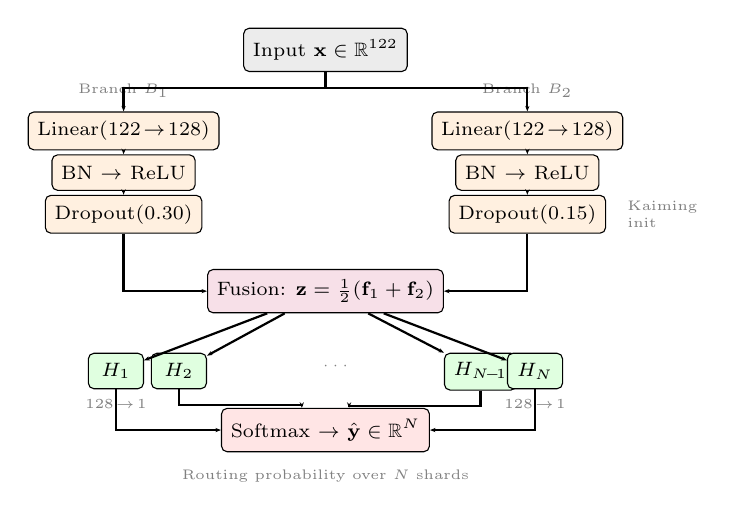
\begin{tikzpicture}[
    node distance=0.4cm and 0.6cm,
    block/.style={rectangle, draw, fill=blue!8, minimum width=1.6cm, minimum height=0.55cm, align=center, font=\scriptsize, rounded corners=2pt},
    branchblock/.style={rectangle, draw, fill=orange!12, minimum width=1.4cm, minimum height=0.45cm, align=center, font=\scriptsize, rounded corners=2pt},
    headblock/.style={rectangle, draw, fill=green!12, minimum width=0.7cm, minimum height=0.45cm, align=center, font=\scriptsize, rounded corners=2pt},
    arr/.style={-{Stealth[length=2pt]}, thick},
    dasharr/.style={-{Stealth[length=2pt]}, thick, dashed, gray},
    lbl/.style={font=\tiny, text=gray}
]

% Input
\node[block, fill=gray!15] (input) {Input $\mathbf{x} \in \mathbb{R}^{122}$};

% Branches
\node[branchblock, below left=0.5cm and 0.3cm of input] (b1lin) {Linear$(122 \!\to\! 128)$};
\node[branchblock, below=0.05cm of b1lin] (b1bn) {BN $\to$ ReLU};
\node[branchblock, below=0.05cm of b1bn] (b1drop) {Dropout$(0.30)$};

\node[branchblock, below right=0.5cm and 0.3cm of input] (b2lin) {Linear$(122 \!\to\! 128)$};
\node[branchblock, below=0.05cm of b2lin] (b2bn) {BN $\to$ ReLU};
\node[branchblock, below=0.05cm of b2bn] (b2drop) {Dropout$(0.15)$};

% Branch labels
\node[lbl, above=0.05cm of b1lin] {Branch $B_1$};
\node[lbl, above=0.05cm of b2lin] {Branch $B_2$};

% Fusion
\node[block, fill=purple!12, below=0.7cm of input, yshift=-1.8cm] (fuse) {Fusion: $\mathbf{z} = \frac{1}{2}(\mathbf{f}_1 + \mathbf{f}_2)$};

% Heads
\node[headblock, below left=0.5cm and 0.8cm of fuse] (h1) {$H_1$};
\node[headblock, below left=0.5cm and 0.0cm of fuse] (h2) {$H_2$};
\node[lbl, below=0.5cm of fuse, xshift=0.15cm] (dots) {$\cdots$};
\node[headblock, below right=0.5cm and 0.0cm of fuse] (hn1) {$H_{N\!-\!1}$};
\node[headblock, below right=0.5cm and 0.8cm of fuse] (hn) {$H_N$};

% Each head label
\node[lbl, below=0.01cm of h1] {\tiny $128\!\to\!1$};
\node[lbl, below=0.01cm of hn] {\tiny $128\!\to\!1$};

% Softmax output
\node[block, fill=red!10, below=1.2cm of fuse] (softmax) {Softmax $\to$ $\hat{\mathbf{y}} \in \mathbb{R}^N$};

% Output label
\node[lbl, below=0.1cm of softmax] {Routing probability over $N$ shards};

% Arrows
\draw[arr] (input.south) -- ++(0,-0.2) -| (b1lin.north);
\draw[arr] (input.south) -- ++(0,-0.2) -| (b2lin.north);
\draw[arr] (b1lin) -- (b1bn);
\draw[arr] (b1bn) -- (b1drop);
\draw[arr] (b2lin) -- (b2bn);
\draw[arr] (b2bn) -- (b2drop);
\draw[arr] (b1drop.south) |- (fuse.west);
\draw[arr] (b2drop.south) |- (fuse.east);
\draw[arr] (fuse) -- (h1);
\draw[arr] (fuse) -- (h2);
\draw[arr] (fuse) -- (hn1);
\draw[arr] (fuse) -- (hn);
\draw[arr] (h1.south) |- (softmax.west);
\draw[arr] (h2.south) -- ++(0,-0.2) -| ([xshift=-0.3cm]softmax.north);
\draw[arr] (hn1.south) -- ++(0,-0.2) -| ([xshift=0.3cm]softmax.north);
\draw[arr] (hn.south) |- (softmax.east);

% Kaiming init annotation
\node[lbl, right=0.15cm of b2drop, align=left] {Kaiming\\init};

\end{tikzpicture}%
}
\caption{EMH-DNN architecture. Two parallel branches with complementary dropout extract diverse features, fused into a shared representation $\mathbf{z}$. Per-client heads $H_k$ produce scalar logits, normalized via softmax into a routing probability over $N$ shards.}
\label{fig:arch}
\end{figure}

\subsubsection{Parallel Feature Extraction}

The network core consists of two parallel branches $B_1$ and $B_2$ processing $\mathbf{x} \in \mathbb{R}^d$ simultaneously (Fig.~\ref{fig:arch}). Let $\mathbf{W}_1, \mathbf{W}_2 \in \mathbb{R}^{h \times d}$ denote their weight matrices ($h = 128$). \emph{Why two branches?} In non-IID federated settings, a single feature extractor risks overfitting to the local distribution of whichever client dominates aggregation. Dual branches with \emph{complementary dropout rates} address this: $B_1$ applies higher dropout (rate $p$), which acts as an implicit ensemble and promotes generalized, distributed representations~\cite{karimireddy2022bucketing}; $B_2$ uses lower dropout ($0.5p$), preserving fine-grained features that $B_1$ may discard. Their fusion combines robustness with fidelity:
\begin{equation}
\mathbf{z} = \frac{1}{2}\big(\phi(\mathbf{W}_1 \mathbf{x}) + \phi(\mathbf{W}_2 \mathbf{x})\big)
\label{eq:fusion}
\end{equation}
where $\phi(\cdot)$ denotes the pipeline of linear transformation, batch normalization, ReLU, and branch-specific dropout. Weights are initialized via Kaiming normal. The specific dropout rates are reported in Section~\ref{sec:config}.

\subsubsection{Client-Specific Multi-Head Output}

The shared representation $\mathbf{z}$ feeds into $N$ distinct output heads $\{H_1, \ldots, H_N\}$, one per client shard. Each head $H_k: \mathbb{R}^h \rightarrow \mathbb{R}$ produces a scalar logit, and the concatenated outputs are normalized via softmax to yield a routing probability distribution over shards:
\begin{equation}
\mathbf{y} = \text{Softmax}\big[H_1(\mathbf{z}),\; H_2(\mathbf{z}),\; \ldots,\; H_N(\mathbf{z})\big]^\top
\label{eq:heads}
\end{equation}
where $\mathbf{y}[j]$ represents the predicted fraction of relevant data residing on shard $j$.

\subsubsection{Trust-Weighted Aggregation}

To limit Sybil influence during model aggregation, base weights $\alpha_k$ (proportional to data size) are scaled by a nonlinear trust-dependent factor. Because trust scores satisfy $\tau_k \in [0, 1]$, raising them to a power $p > 1$ amplifies the gap between high- and low-trust clients. The study use cubic scaling for probationary clients and quadratic for trusted ones:
% FIX 6: cases text shortened to fit one column.
\begin{equation}
\alpha_k^{(trust)} = \alpha_k \cdot 
\begin{cases}
\tau_k^3 & \tau_k < \tau_{min} \;\text{(probationary)} \\
\tau_k^2 & \tau_k \geq \tau_{min} \;\text{(trusted)}
\end{cases}
\label{eq:agg}
\end{equation}

The stronger cubic suppression for probationary clients ensures that newcomers---who have not yet demonstrated sustained honest behavior---contribute minimally to aggregation even if they pass PoC screening, following the principle that initial trust must be earned, not assumed~\cite{cao2021fltrust}.

\subsubsection{Deployment in the Federated Setting}

The \emph{server} instantiates a single global EMH-DNN with $N$ output heads matching the number of client shards. Each round, eligible client $k$ receives a deep copy of $\mathbf{w}_g^{(t)}$ and trains locally on its private SIFT shard $\mathcal{D}_k$ for 3 epochs. Because the training labels are normalized routing distributions over \emph{all} $N$ shards (Section~\ref{sec:task}), client $k$'s loss function produces gradients for the shared branches ($B_1$, $B_2$) and all $N$ heads simultaneously: the ground-truth vector $\mathbf{y}[i]$ assigns nonzero probability to every shard containing at least one of the query's top-1000 neighbors, so the MSE loss naturally propagates learning signal to each head $H_j$ in proportion to shard $j$'s true neighbor density. In practice, the dominant gradient flows to client $k$'s own head (which holds the largest neighbor share), while the remaining heads receive weaker but nonzero supervision. Each head is a single linear layer ($128 \to 1$), so the $N$-head overhead is $\mathcal{O}(Nh)$ parameters---negligible relative to the shared branches when $N$ is small (4--8 in our experiments); for larger federations, head pruning or sparse communication could further reduce this cost.

This architectural separation ensures: (i)~the shared encoder converges to a universal embedding across shards, and (ii)~the per-head isolation \emph{mitigates} catastrophic forgetting \emph{at the routing layer}, since each shard's routing knowledge is maintained in a dedicated head. Forgetting in the shared branches due to non-IID updates remains possible and is addressed by trust-weighted aggregation (Eq.~\ref{eq:agg}), which limits low-trust clients' influence on the shared representation. Validated updates are committed to the blockchain. To trigger Layer~2 rollback, each committee member independently evaluates the updated global model on its own local test partition; if the median Recall@1000 across committee members drops below the safety margin $\delta_{drop}$, the slashing and rollback protocol (Section~2.2) is activated.

\subsection{Protocol Summary}

Algorithm~\ref{alg:protocol} summarizes the complete protocol.

% FIX 4: The long \STATE line with \hfill caused right-margin overflow.
%         Split it into two lines and remove the \hfill spacer.
\begin{algorithm}[t]
\caption{Secure Two-Layer Federated Learning}
\label{alg:protocol}
\scriptsize
\begin{algorithmic}[1]
\STATE \textbf{Initialize:} Model $\mathbf{w}_0$, trust $\tau_k^{(0)} = 0.3\;\forall k$, stakes $S$
\FOR{round $t = 1, \ldots, T$}
    \STATE \textit{// Layer 1: Consensus}
    \STATE Elect committee $\mathcal{C}^{(t)}$ via score-based selection
    \STATE $\mathcal{P}_{valid} \leftarrow \emptyset$
    \FOR{each eligible client $k$ \textbf{in parallel}}
        \STATE $\mathbf{w}_k \leftarrow \text{LocalTrain}(\mathbf{w}_g^{(t-1)}, \mathcal{D}_k)$ using EMH-DNN
        \STATE Compute $S_{PoC}(k)$ per Eq.~(\ref{eq:poc})
        \IF{$S_{PoC}(k) \geq \delta_{th}$}
            \STATE Committee validates; accept if $\geq 2/3$ approve
            \IF{accepted}
                \STATE $\mathcal{P}_{valid} \leftarrow \mathcal{P}_{valid} \cup \{(\mathbf{w}_k, S_{combined}(k))\}$
            \ENDIF
        \ENDIF
    \ENDFOR
    \STATE \textit{// Trust-weighted aggregation:}
    \STATE $\mathbf{w}_g^{(t+1)} \leftarrow
           \sum_{k \in \mathcal{P}_{valid}} \alpha_k^{(trust)} \cdot \mathbf{w}_k$
    \STATE Mine block $B_t$ with validated updates
    \STATE \textit{// Layer 2: Economic Security}
    \STATE Each committee member evaluates $\text{Acc}_t$ on its private
           local test partition; compute median on-chain.
    \IF{$\text{Acc}_t < \text{Acc}_{t-1} - \delta_{drop}$}
        \STATE Rollback to $\mathbf{w}_g^{(t-1)}$; slash $\mathcal{C}^{(t)}$;
               set $\tau_j \leftarrow 0$
    \ELSE
        \STATE Update trust per Eq.~(\ref{eq:trust}); commit $B_t$
    \ENDIF
\ENDFOR
\end{algorithmic}
\end{algorithm}

%=====================================================
\section{Experimental Evaluation}
%=====================================================

\subsection{Experimental Setup}

\subsubsection{Task, Dataset, and Evaluation Metric}
\label{sec:task}

The study evaluate the framework on an \emph{approximate nearest neighbor (ANN) routing} task---a core operation in large-scale retrieval systems where a database is sharded across distributed clients.

\textbf{Dataset.} The research use the SIFT1B benchmark~\cite{jegou2008pq}, a standard billion-scale dataset of Scale-Invariant Feature Transform (SIFT) descriptors widely used for evaluating ANN search. SIFT descriptors are 128-dimensional gradient-histogram vectors extracted from image keypoints; our preprocessed subset uses 122-dimensional vectors. The dataset is partitioned across $N$ client shards with high data skew (non-uniform shard sizes and distributional heterogeneity) to simulate realistic non-IID federated scenarios. Two configurations are tested: $N \in \{4, 8\}$, with 50\% of clients designated as Sybil attackers.

\textbf{Learning task.} Given a query vector $\mathbf{x} \in \mathbb{R}^{122}$, the true top-1000 nearest neighbors are distributed across the $N$ shards. The ground-truth label $\mathbf{y}^{raw}[i] \in \mathbb{Z}^N$ records the count of true top-1000 neighbors on each shard (summing to 1000), and is row-normalized to a probability distribution $\mathbf{y}[i] = \mathbf{y}^{raw}[i] / 1000$. The EMH-DNN learns to predict the routing distribution $\hat{\mathbf{y}}[i]$ by minimizing MSE loss against $\mathbf{y}[i]$, so that queries can be routed to the shard(s) most likely to contain relevant neighbors.

\textbf{Recall@1000.} Following standard retrieval evaluation, Recall@1000 is the fraction of true top-1000 neighbors found in probed shards: $\text{Recall@1000} = \sum_{j \in \mathcal{S}_K} \mathbf{y}^{raw}[i][j] \,/\, 1000$, where $\mathcal{S}_K$ contains the $K$ shards with highest predicted probability. The study report top-1 routing ($K=1$): the query is sent to $\arg\max_j \hat{\mathbf{y}}[j]$ only, and recall measures how many true neighbors reside on that shard.

\subsubsection{Model and Protocol Configuration}
\label{sec:config}

The EMH-DNN (Fig.~\ref{fig:arch}) is trained with MSE loss using SGD (lr $= 0.01$, momentum $= 0.9$) for 3 local epochs per round with batch size 128. Committees comprise 30\% of eligible clients. Trust: $\tau_k^{(0)} = 0.3$, $\tau_{min} = 0.45$, $r_{reward} = 0.02$ ($0.05$ probationary), $r_{penalty} = 0.15$. PoC: $\gamma_1 = 0.4$, $\gamma_2 = 0.4$, $\gamma_3 = 0.2$; $\delta_{th}$ adapts from $0.02$ to $0.1$. Layer~2: $\delta_{drop} = 0.05$, $S_{min} = 10.0$, $P_{penalty} = 5.0$.

\subsubsection{Attack Model}

Adversarial clients execute a coordinated 50\% Sybil attack using \emph{sign-flip} poisoning (negating gradient directions to maximally degrade the global model) combined with free-riding (zero/minimal updates), while attempting to maintain trust scores above the participation threshold.

\subsection{Performance Analysis}

\subsubsection{Global Model Convergence}

Despite heavy adversarial presence, the system demonstrated robust convergence over 20 communication rounds (Table~\ref{tab:results}). The global model achieved Recall@1000 of \textbf{93.93\%} for $N = 4$ and \textbf{93.72\%} for $N = 8$ under top-1 shard routing. MSE test loss decreased consistently to $1.81 \times 10^{-3}$ ($N = 4$) and $8.12 \times 10^{-4}$ ($N = 8$), confirming that the decentralized committee validation and trust-weighted aggregation successfully filtered sign-flip poisoned updates.

\begin{table}[t]
\centering
\caption{Performance and Security Metrics on SIFT Dataset (20 Rounds, 50\% Sybil Attack)}
\label{tab:results}
\begin{tabular}{lcc}
\toprule
\textbf{Metric} & \textbf{$N=4$} & \textbf{$N=8$} \\
\midrule
\multicolumn{3}{l}{\textit{Model Utility}} \\
Final Test Recall@1000 & 93.93\% & 93.72\% \\
Final Test Loss (MSE) & 0.0018 & 0.0008 \\
\midrule
\multicolumn{3}{l}{\textit{Security \& Trust}} \\
Honest Trust ($\tau_{honest}$) & 0.41 & 0.39 \\
Sybil Trust ($\tau_{sybil}$) & 0.15 & 0.15 \\
Peak ASR (Round 1) & 100.0\% & 100.0\% \\
Final ASR (Round 20) & \textbf{0.0\%} & \textbf{0.0\%} \\
Total Sybil Updates Accepted & 2 & 4 \\
\bottomrule
\end{tabular}
\end{table}

\subsubsection{Sybil Resistance and Trust Dynamics}

In Round~1, the system operated in a ``trust-but-verify'' mode, resulting in a 100\% Attack Success Rate as initial Sybil updates were tentatively accepted (2~updates for $N=4$, 4~updates for $N=8$). However, Layer~2 mechanisms responded immediately: by Round~2, the ASR dropped to \textbf{0.0\%} and remained there for all subsequent rounds. Honest clients stabilized at $\tau \approx 0.41$ ($N=4$) and $\tau \approx 0.39$ ($N=8$), while Sybil clients were penalized from $\tau = 0.3$ to the minimum floor of $\tau = 0.15$, effectively locking them out of committee participation. The trust dynamics demonstrate the effectiveness of combining PoP-based identity verification with economic penalties.

\subsubsection{Committee Fairness}

Honest clients served as committee members in 4--5~rounds ($N=4$) and 2--4~rounds ($N=8$), demonstrating balanced validation responsibilities. Sybil clients were excluded after initial penalization, confirming the trust-weighted election prevents adversarial concentration of power.

\subsection{Comparison with State-of-the-Art}

Table~\ref{tab:sota} benchmarks the proposed framework against established standards, including VeryFL's verifiable aggregation~\cite{li2025veryfl}, FL-Defender's gradient-based defenses~\cite{jebreel2023fl}, and applications in critical infrastructure domains~\cite{alashhab2024enhancing, asiri2023understanding, jayagopal2023intrusion}.

\begin{table}[t]
\centering
\caption{Comparison with State-of-the-Art Security Standards}
\label{tab:sota}
\scriptsize
\setlength{\tabcolsep}{3pt}
\begin{tabular}{lccc}
\toprule
\textbf{Metric} & \textbf{Industry}~\cite{asiri2023understanding,jayagopal2023intrusion} & \textbf{Research}~\cite{jebreel2023fl,huang2024federated,alashhab2024enhancing} & \textbf{Ours} \\
\midrule
\multicolumn{4}{l}{\textit{Security Resilience}} \\
ASR & $< 10\%$ & $< 1\%$ & \textbf{0.0\%} \\
Attack Tolerance & 20\%--33\% & 33\%--45\% & \textbf{50\%} \\
Sybil Handling & Filtering & Statistical & \textbf{Rej.\ + Banned} \\
\midrule
\multicolumn{4}{l}{\textit{Model Utility}} \\
Accuracy Drop & $< 5\%$ & $< 3\%$ & $\approx$ \textbf{0.0\%} \\
Final Recall@1000 & $> 95\%$ & $> 98\%$ & \textbf{93.93\%} \\
Comp.\ Overhead & High & Moderate & \textbf{Low} \\
\bottomrule
\end{tabular}
\end{table}

The proposed framework achieves \textbf{0.0\%} ASR, surpassing both industry ($<10\%$) and research ($<1\%$) benchmarks, with \textbf{50\%} attack tolerance exceeding the 33\%--45\% threshold typical of Byzantine-robust methods~\cite{huang2024federated}. Unlike statistical filtering approaches, Layer~2 \emph{rejects and permanently bans} malicious clients through economic slashing and state rollback, while maintaining low computational overhead due to the lightweight median-voting consensus.

%=====================================================
\section{Discussion and Limitations}
%=====================================================

The two-layer design provides complementary security. For instance, Layer~1 offers proactive defense through trust-gated participation and peer validation. Likewise, Layer~2 detects and reverses poisoning that evades initial screening. Subsequently, replacing global validation sets with peer-to-peer evaluation on private local data, the framework preserves FL's privacy guaranty an improvement over systems such as BlockFL~\cite{kim2019blockfl}. The staking mechanism ($P_{penalty} = 5.0$ against $S_{min} = 10.0$) eliminates half a validator's stake per slashing event, with trust reset to zero permanently excluding them, making sustained collusion prohibitively expensive.

Several limitations warrant acknowledgment. The framework has been evaluated only on small networks ($N \leq 8$); large-scale deployments may require hierarchical committee architectures and techniques to manage the linearly growing $N$-head communication cost (e.g., head pruning, sparse updates, or federated distillation). Similarly, the multi-head design mitigates catastrophic forgetting at the routing layer but does not fully prevent representation drift in the shared branches under extreme non-IID heterogeneity; complementary techniques such as FedProx regularization could strengthen this. The system assumes PoP-based trust initialization, which may be challenging in fully anonymous environments. The staking requirement creates entry barriers for resource-constrained participants, and the peer validation process introduces communication overhead compared to centralized approaches. Future work includes adaptive trust initialization for trustless bootstrapping, differential privacy guarantees for peer validation, tiered incentive mechanisms balancing security with accessibility, and extending the framework beyond EMH-DNN. All intensive operations — training, PoC scoring, and evaluation — execute off-chain; only contribution scores, model hashes, and stake transactions are committed on-chain, keeping overhead minimal while preserving privacy.

%=====================================================
\section{Conclusion}
%=====================================================

The paper presented a two-layer blockchain framework for secure decentralized FL. Likewise, Layer~1 eliminates reliance on global validation sets through PoP identity governance and decentralized median-voting consensus. Subsequently, Layer~2 introduces economic accountability via staking, slashing, and blockchain-based rollback. More precisely, that renders poisoning both economically irrational and technically reversible. The EMH-DNN architecture supports non-IID robustness through parallel feature extraction and client-specific output heads.

Experimental evaluation on an ANN routing task over the SIFT1B benchmark confirms $\sim$93.8\% Recall@1000 under a 50\% Sybil attack while reducing ASR from 100\% to 0.0\% within a single round of retroactive correction. These results establish that privacy-preserving, economically accountable federated learning is achievable in adversarial decentralized environments.

%=====================================================
% References
%=====================================================

\begin{thebibliography}{00}

\bibitem{li2020blockchain}
Y.~Li, C.~Chen, N.~Liu, H.~Huang, Z.~Zheng, and Q.~Yan,
``A blockchain-based decentralized federated learning framework with committee consensus,''
\textit{IEEE Network}, vol.~35, no.~1, pp.~234--241, 2021.

\bibitem{kim2020ondevice}
H.~Kim, J.~Park, M.~Bennis, and S.-L.~Kim,
``On-device federated learning via blockchain and its latency analysis,''
\textit{IEEE Trans. Cogn. Commun. Netw.}, vol.~6, no.~3, pp.~1198--1211, 2020.

\bibitem{kim2019blockfl}
H.~Kim, J.~Park, M.~Bennis, and S.-L.~Kim,
``Blockchained on-device federated learning,''
\textit{IEEE Commun. Lett.}, vol.~24, no.~6, pp.~1279--1283, 2020.

\bibitem{liu2020flchain}
Y.~Liu, Y.~Ai, S.~Zhang, Z.~Li, G.~Gui, and H.~Wang,
``FLChain: A blockchain-based federated learning system,''
in \textit{Proc. IEEE Int. Conf. Commun. (ICC)}, 2020, pp.~1--6.

\bibitem{shayan2021biscotti}
M.~Shayan, C.~Fung, C.~J.~M.~Yoon, and I.~Beschastnikh,
``Biscotti: A blockchain system for private and secure federated learning,''
\textit{IEEE Trans. Parallel Distrib. Syst.}, vol.~33, no.~7, pp.~1513--1525, 2021.

\bibitem{li2025veryfl}
Y.~Li, T.~Lai \textit{et al.},
``VeryFL: A verify federated learning framework embedded with blockchain,''
\textit{arXiv:2311.15617}, 2023.

\bibitem{peng2022vfchain}
Z.~Peng, J.~Xu, X.~Chu, S.~Gao, Y.~Yao, R.~Gu, and Y.~Tang,
``VFChain: Enabling verifiable and auditable federated learning via blockchain systems,''
\textit{IEEE Trans. Netw. Sci. Eng.}, vol.~9, no.~1, pp.~173--186, 2022.

\bibitem{bellachia2025verifbfl}
A.~A.~Bellachia \textit{et al.},
``VerifBFL: Leveraging zk-SNARKs for a verifiable blockchained federated learning,''
\textit{arXiv:2501.04319}, 2025.

\bibitem{jiang2024bfl}
Y.~Jiang \textit{et al.},
``Blockchained federated learning for Internet of Things: A comprehensive survey,''
\textit{ACM Comput. Surv.}, vol.~56, no.~10, 2024.

\bibitem{li2022bflsurvey}
D.~Li \textit{et al.},
``Blockchain for federated learning toward secure distributed machine learning systems: A systemic survey,''
\textit{Soft Comput.}, vol.~26, no.~9, pp.~4423--4440, 2022.

\bibitem{douceur2002sybil}
J.~R.~Douceur,
``The Sybil attack,''
in \textit{Proc. Int. Workshop Peer-to-Peer Syst. (IPTPS)}, 2002, pp.~251--260.

\bibitem{borge2017pop}
M.~Borge, E.~Kokoris-Kogias, P.~Jovanovic, and B.~Ford,
``Proof-of-personhood: Redemocratizing permissionless cryptocurrencies,''
in \textit{Proc. IEEE European Symp. Security Privacy Workshops (EuroS\&PW)}, 2017, pp.~23--26.

\bibitem{siddarth2020pop}
D.~Siddarth, S.~Ivliev, S.~Siri, and P.~Berman,
``Who watches the watchmen? A review of subjective approaches for Sybil-resistance in proof of personhood protocols,''
\textit{Frontiers Blockchain}, vol.~3, Art.~590171, 2020.

\bibitem{adler2024phc}
S.~Adler, Z.~Hitzig, S.~Jain \textit{et al.},
``Personhood credentials: Artificial intelligence and the value of privacy-preserving tools to distinguish who is real online,''
\textit{arXiv:2408.07892}, 2024.

\bibitem{fung2020foolsgold}
C.~Fung, C.~J.~M.~Yoon, and I.~Beschastnikh,
``The limitations of federated learning in Sybil settings,''
in \textit{Proc. 23rd Int. Symp. Research Attacks, Intrusions Defenses (RAID)}, USENIX, 2020, pp.~301--316.

\bibitem{samy2023fedsybil}
A.~E.~Samy and \v{S}.~Girdzijauskas,
``Mitigating Sybil attacks in federated learning,''
in \textit{Information Security Practice and Experience (ISPEC)}, LNCS, vol.~14341, 2023, pp.~33--48.

\bibitem{fang2020local}
M.~Fang, X.~Cao, J.~Jia, and N.~Z.~Gong,
``Local model poisoning attacks to Byzantine-robust federated learning,''
in \textit{Proc. 29th USENIX Security Symp.}, 2020, pp.~1605--1622.

\bibitem{blanchard2017krum}
P.~Blanchard, E.~M.~El~Mhamdi, R.~Guerraoui, and J.~Stainer,
``Machine learning with adversaries: Byzantine tolerant gradient descent,''
in \textit{Proc. Adv. Neural Inf. Process. Syst. (NeurIPS)}, vol.~30, 2017.

\bibitem{yin2018byzantine}
D.~Yin, Y.~Chen, R.~Kannan, and P.~Bartlett,
``Byzantine-robust distributed learning: Towards optimal statistical rates,''
in \textit{Proc. Int. Conf. Mach. Learn. (ICML)}, 2018, pp.~5650--5659.

\bibitem{cao2021fltrust}
X.~Cao, M.~Fang, J.~Liu, and N.~Z.~Gong,
``FLTrust: Byzantine-robust federated learning via trust bootstrapping,''
in \textit{Proc. Network Distrib. Syst. Security Symp. (NDSS)}, 2021.

\bibitem{nguyen2022flame}
T.~D.~Nguyen, P.~Rieger, H.~Chen \textit{et al.},
``FLAME: Taming backdoors in federated learning,''
in \textit{Proc. 31st USENIX Security Symp.}, 2022, pp.~1415--1432.

\bibitem{jebreel2023fl}
N.~M.~Jebreel and J.~Domingo-Ferrer,
``FL-Defender: Combating targeted attacks in federated learning,''
\textit{Knowl.-Based Syst.}, vol.~260, Art.~110178, 2023.

\bibitem{huang2024federated}
W.~Huang, M.~Ye, Z.~Shi, G.~Wan, H.~Li, B.~Du, and Q.~Yang,
``Federated learning for generalization, robustness, fairness: A survey and benchmark,''
\textit{IEEE Trans. Pattern Anal. Mach. Intell.}, vol.~46, no.~12, 2024.

\bibitem{karimireddy2022bucketing}
S.~P.~Karimireddy, L.~He, and M.~Jaggi,
``Byzantine-robust learning on heterogeneous datasets via bucketing,''
in \textit{Proc. Int. Conf. Learn. Representations (ICLR)}, 2022.

\bibitem{karimireddy2021history}
S.~P.~Karimireddy, L.~He, and M.~Jaggi,
``Learning from history for Byzantine robust optimization,''
in \textit{Proc. Int. Conf. Mach. Learn. (ICML)}, 2021, pp.~5311--5319.

\bibitem{baruch2019little}
G.~Baruch, M.~Baruch, and Y.~Goldberg,
``A little is enough: Circumventing defenses for distributed learning,''
in \textit{Proc. Adv. Neural Inf. Process. Syst. (NeurIPS)}, 2019.

\bibitem{buterin2019casper}
V.~Buterin and V.~Griffith,
``Casper the friendly finality gadget,''
\textit{arXiv:1710.09437}, 2019.

\bibitem{wood2014polkadot}
G.~Wood,
``Polkadot: Vision for a heterogeneous multi-chain framework,''
Polkadot White Paper, 2016.

\bibitem{weng2021deepchain}
J.~Weng, J.~Weng, J.~Zhang, M.~Li, Y.~Zhang, and W.~Luo,
``DeepChain: Auditable and privacy-preserving deep learning with blockchain-based incentive,''
\textit{IEEE Trans. Dependable Secure Comput.}, vol.~18, no.~5, pp.~2438--2455, 2021.

\bibitem{kang2019incentive}
J.~Kang, Z.~Xiong, D.~Niyato, S.~Xie, and J.~Zhang,
``Incentive mechanism for reliable federated learning: A joint optimization approach to combining reputation and contract theory,''
\textit{IEEE Internet Things J.}, vol.~6, no.~6, pp.~10700--10714, 2019.

\bibitem{desai2021blockfla}
H.~B.~Desai, M.~S.~Ozdayi, and M.~Kantarcioglu,
``BlockFLA: Accountable federated learning via hybrid blockchain architecture,''
in \textit{Proc. ACM Conf. Data Appl. Security Privacy (CODASPY)}, 2021, pp.~101--112.

\bibitem{cao2023fedrecover}
X.~Cao, J.~Jia, Z.~Zhang, and N.~Z.~Gong,
``FedRecover: Recovering from poisoning attacks in federated learning using historical information,''
in \textit{Proc. IEEE Symp. Security Privacy (S\&P)}, 2023, pp.~1366--1383.

\bibitem{jiang2024crab}
Y.~Jiang, J.~Shen, Z.~Liu, C.~Tan, and K.-Y.~Lam,
``Towards efficient and certified recovery from poisoning attacks in federated learning,''
\textit{arXiv:2401.08216}, 2024.

\bibitem{wu2023fedgame}
C.~Wu \textit{et al.},
``FedGame: A game-theoretic defense against backdoor attacks in federated learning,''
in \textit{Proc. Adv. Neural Inf. Process. Syst. (NeurIPS)}, 2023.

\bibitem{alashhab2024enhancing}
Z.~R.~Alashhab \textit{et al.},
``Enhancing DDoS detection in SDN using federated learning,''
\textit{IEEE Access}, 2024.

\bibitem{asiri2023understanding}
M.~Asiri \textit{et al.},
``Understanding indicators of compromise against cyber-attacks in industrial control systems,''
\textit{Electronics}, 2023.

\bibitem{jayagopal2023intrusion}
R.~Jayagopal \textit{et al.},
``Intrusion detection system for IoT-based smart environments,''
\textit{Sensors}, 2023.

\bibitem{jegou2008pq}
H.~J\'{e}gou, M.~Douze, and C.~Schmid,
``Product quantization for nearest neighbor search,''
\textit{IEEE Trans. Pattern Anal. Mach. Intell.}, vol.~33, no.~1, pp.~117--128, 2011.

\end{thebibliography}

\end{document}